\documentclass[aps,prd,onecolumn,notitlepage,nofootinbib,superscriptaddress,altaffilletter,floatfix]{revtex4-1}

%\documentclass[twocolumn,superscriptaddress,showpacs,preprintnumbers,amsmath,amssymb]{revtex4}
%\documentclass[,showpacs,preprintnumbers,amsmath,amssymb]{revtex4}

%\bibliographystyle{unsrt}
%ieeetr
\usepackage{graphicx}% Include figure files
\usepackage{float}
\usepackage{amssymb}
\usepackage{amsmath}
\usepackage{longtable}
\usepackage{color}
\usepackage{hyperref}

% Bibliography style
%%\bibliographystyle{abbrvnat}
\bibliographystyle{apsrev}

\usepackage{soul}
\newcommand{\repr}[1]{{\color{red}[#1]}}
\newcommand{\strike}[1]{\textrm{\color{red}\st{#1}}}
\newcommand{\replace}[2]{\strike{#1} \textrm{$\rightarrow$} {\color{green}#2}}

\newcommand{\tStart}{t_0}
\newcommand{\tEvent}{t_{\mathrm{event}}}
\newcommand{\tMerger}{t_{\mathrm{M}}}
\newcommand{\freq}{f_0}

\newcommand{\parA}{{\mathcal A}}
\newcommand{\As}{\parA_{\mathrm{s}}}
\newcommand{\Ac}{\parA_{\mathrm{c}}}

\newcommand{\xs}{x_{\mathrm{s}}}
\newcommand{\xc}{x_{\mathrm{c}}}
\newcommand{\xvec}{\vec{x}}

\newcommand{\hs}{h_\mathrm{s}}
\newcommand{\hc}{h_\mathrm{c}}
\newcommand{\hexp}{h_{\mathrm{exp}}}
\newcommand{\Is}{I_{\mathrm{s}}}
\newcommand{\Ic}{I_{\mathrm{c}}}
\newcommand{\Isc}{I_{\mathrm{sc}}}
\newcommand{\M}{\mathcal{M}}
\newcommand{\Mss}{\M_{\mathrm{ss}}}
\newcommand{\Mcc}{\M_{\mathrm{cc}}}
\newcommand{\Msc}{\M_{\mathrm{sc}}}

\newcommand{\Dt}{\Delta t}
\newcommand{\scalar}[2]{\left\langle #1\middle|#2\right\rangle}
\newcommand{\Hyp}{\mathcal{H}}
\newcommand{\HypG}{\Hyp_{\mathrm{G}}}
\newcommand{\HypS}{\Hyp_{\mathrm{S}}}
\newcommand{\prob}[2]{P\left(#1\middle|#2\right)}
\newcommand{\FT}[1]{\widetilde{#1}}
\newcommand{\parE}{\lambda}
\newcommand{\BSG}{B_{\mathrm{S/G}}}
\newcommand{\Lr}{\mathcal{L}}
\newcommand{\Ord}[1]{\mathcal{O}\left(#1\right)}

\newcommand{\MP}{{\mathrm{MP}}}

\newcommand{\Sn}{\mathcal{S}}
\newcommand{\SX}{S_X}
\newcommand{\Ndet}{N_{\mathrm{det}}}
\newcommand{\sig}{{\mathrm{sig}}}
\newcommand{\Gam}{\gamma}
\newcommand{\eye}{\mathbb{I}}
\newcommand{\Fab}{F}
\newcommand{\F}{\mathcal{F}}
\newcommand{\trace}[1]{\mathrm{tr}#1}
%% ---------- Units ----------
\newcommand{\ms}{\mathrm{ms}}
\newcommand{\Hz}{\mathrm{Hz}}
\renewcommand{\sec}{\mathrm{s}}
%%% Local Variables:
%%% mode: latex
%%% TeX-master: t
%%% End:

\input{git_tag.tex}

\newcommand{\dcc}{LIGO-T1500618-v4pre}

\begin{document}

\title{Bayesian QNM search on black hole ringdown modes (applied to GW150914)}

%% \title{Template-based investigations to study the parameter-space metric for known continuous
%% wave sources in binary systems}

\author{Reinhard Prix}
\altaffiliation{Reinhard.Prix@ligo.org}
\affiliation{Max-Planck-Institut f\"ur Gravitationsphysik, Albert-Einstein-Institut, D-30167 Hannover, Germany}
\date{\commitDATE; \commitIDshort-\commitSTATUS; \href{https://dcc.ligo.org/LIGO-T1500618}{\dcc}}
%\parbox[c]{1em}{\textcolor{red}{DRAFT}}


\begin{abstract}
  We quantify the evidence for and estimate the parameters of QNM 'ringdown' in the GW150914 event.
  This is done by Bayesian hypothesis testing and parameter estimation using a QNM ringdown model
  $s(t\ge\tStart) = A\,e^{-\frac{t-\tStart}{\tau}}\cos\left(2\pi \freq (t-\tStart) + \phi_0\right)$ with unknown amplitude $A$, initial phase $\phi_0$,
  frequency $\freq$ and decay time $\tau$, as a function of the QNM start-time $\tStart$.
  Using a Gaussian-isotropic prior on $\{\As=-A\sin\phi_0,\,\Ac=A\cos\phi_0\}$ we can approximate the Bayes factor by analytically marginalizing over
  $\{A,\phi_0\}$, leaving an explicit template search over $\{\freq,\,\tau\}$.
\end{abstract}

%%\pacs{04.80.Nn, 95.55.Ym, 95.75.-z, 97.60.Gb, 07.05.Kf}% PACS, the Physics and Astronomy
\maketitle

\subsection{Changelog}
\label{sec:changelog}

A number of changes compared to the previous version (v3,v3+) that went into the submitted paper (\href{http://arxiv.org/abs/1602.03841}{arXiv:1602.03841}).

\begin{itemize}
\item bug: previous results suffered from a small bug in (old version of) octapps \texttt{FourierTransform} wrapper, which contained an ``off-by-one'' type
  error, leading to slight de-phasing of the data time-series

\item bug: previously the 'SNR-term' in the likelihood $\scalar{s}{s}$ was computed over the full SFT frequency band $[10,2000]\,\Hz$, instead of
  the relevant narrow-banded data $[30,1000]\,\Hz$ actually used in the search-term $\scalar{x}{s}$

\item bug/inconsistency (up to version 'v4-'): I had used a tukey(0.1) window on SFT data (spanning ${[10,2000]}\Hz$) before inv-FFTing into
  time-domain, and then used data starting from 30Hz. At these low frequencies, however, the data was still affected by the Tukey-window (clearly
  visible in the previous PSD estimates). I've now reduced this to tukey(0.02), which is enough to avoid creating spurious time-domain noise, and even
  allowed me to push the low-frequency end down to $20\,\Hz$.

\item expanded used data-range from previously ${[30,1000]}\,\Hz$ to ${[20,1900]}\,\Hz$ (which avoids the lower and upper boundaries near 10Hz and 2000Hz affected by tukey(0.02)-windowing).

\item apply tukey(0.1)-windowing to the $T=8\,$s time-series data before FFTing for whitening: this avoids red-noise artifacts, especially visible in
  L1 whitened spectra in previous versions (up to 'v4-'). Contrary to the frequency domain, none of the data near the start and end is actually used,
  so a wider window is used.

\item PSD estimation: avoid using the central data-segment of $T=8\,\sec$ containing GW150914 (or any injections) to avoid affecting the PSD estimate

\item slight inconsistency: previous results used  $\tMerger = 1126259462.42285$, while the paper stated  $\tMerger = 1126259462.423$
  (rounded to $\ms$). While small, this \emph{does} change the numbers (and posteriors) slightly, especially towards the end ($+7\ms$), due to the
  exponentiall fall-off of the Bayes-factor with offsets from $\tStart$. The new results use the merger time rounded to ms-accuracy as quoted in the
  paper.

\item Improved: use \emph{maximum-posterior} (rather than partially maximum-likelihood) estimate of amplitude parameters and resulting SNR. Essentially
  makes no relevant numerical difference on actual signals, though.

\item Improved: substantial speedup of code: larger sampling of ``off-source'' noise distributions on actual data and on Gaussian white noise

\item Improved: added injection feature of QNM signals, allowing quantified test of accuracy of parameter-estimation and posterior coverage

\item improved iso-probability contour estimation accuracy

\end{itemize}

All results shown in this version of the notes were produced using the ringdown pipeline in
\href{https://git.ligo.org/BlackHole-QNM-Ringdown/Bayesian-QNM-PE-octave}{gitLab}, version
\href{https://git.ligo.org/BlackHole-QNM-Ringdown/Bayesian-QNM-PE-octave/commit/ed4ff88fbe557f371fab4fded258f0b4fe03c67c}{ed4ff88f}.

\newpage
\subsection{Proposed updated statements for PRL "Testing GR" paper}
\label{sec:prop-updat-stat}

Qualitatively these results agree with what was stated and presented in the originally submitted PRL version.
However the numbers and posterior contours are somewhat different.
However, this version is clearly more mature/converged, and more fully tested and characterized, and a number of bugs and possible inconsistencies
have been fixed since v3 (and even v4-).
We therefore propose to update the text and results when re-submitting the paper to PRL in the following way:

\begin{center}
  \parbox{0.7\textwidth}{
    We use 1800s of detector data containing GW150914 from H1 and L1, band-passed to ${[20,1900]}\,\Hz$.
    We assume the signal arrived $7\,\ms$ earlier in L1 compared to H1, and that the amplitude has opposite sign in both detectors. [ref detection paper?]\\
    \ldots\\
    The $90\%$ posterior contour overlaps the GR prediction from
    the IMR waveform after about $\tStart \gtrsim \tMerger + 3\,\ms$, or $\sim10\,M$
    after merger. The corresponding Bayes factor at this point
    is $\log_{10}B \sim 14$ and the MAP waveform SNR is $\sim 8$.
    At $\tStart = \tMerger + 5\,\ms$ the MAP parameters fall within the contour
    predicted in GR for the least-damped QNM, with $\log_{10}B \sim 6.5$
    and SNR\ $\sim 6.5$. At $\tStart = \tMerger + 6.5\,\ms$, or about $\sim20\,M$ after merger,
    the posterior uncertainty becomes quite large, and the Bayes
    factor drops to $\log_{10}B \sim 3.5$ with SNR\ $\sim 4.8$. The signal
    becomes undetectable after about $\tStart \gtrsim \tMerger + 8.5\,\ms$,
    where $B \lesssim 1$.
  }
\end{center}

New posterior contours [the official plot will again be produced by Walter] for selected time-steps (new result on the right, current plot on the
left):\\
\newcommand{\onSourceDir}{./Results/Results-160410-08h23-onSource13-data20Hz-1900Hz-Prior-f200Hz-300Hz-df0.5Hz-tau0.5ms-20.0ms-dtau0.5ms-H2.0-10.0-dH1.0/}
\parbox{\textwidth}{
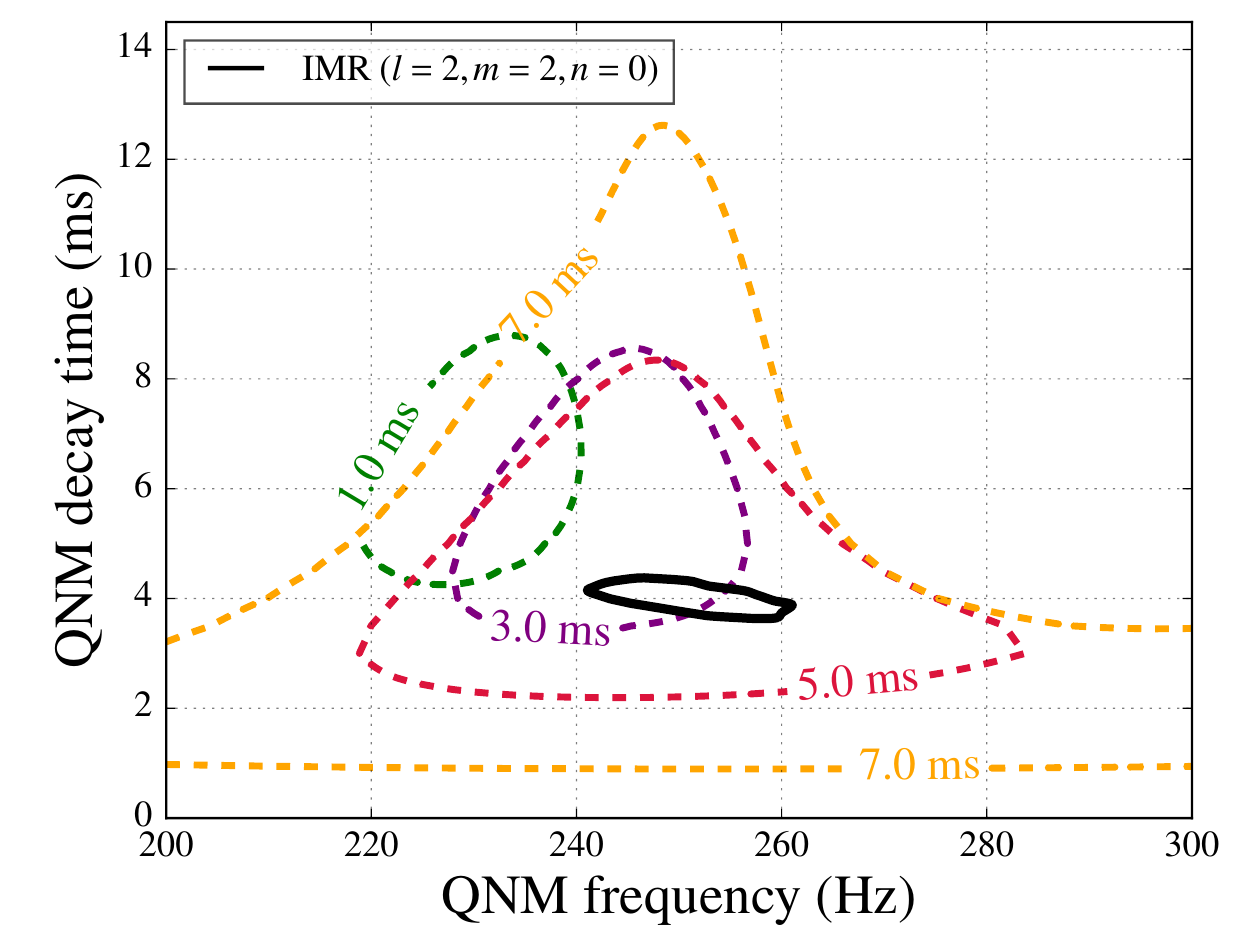
\includegraphics[width=0.49\textwidth]{./QNM-contours-orig.png}
\includegraphics[width=0.49\textwidth]{{\onSourceDir/Posterior-Contours}.pdf}
}

\newpage
%%%%%%%%%%%%%%%%%%%%%%%%%%%%%%%%%%%%%%%%%%%%%%%%%%%%%%%%%%%%%%%%%%%%%%%%%%%%%%%%%%%%%%%
\section{Introduction}
\label{Intro}
%%%%%%%%%%%%%%%%%%%%%%%%%%%%%%%%%%%%%%%%%%%%%%%%%%%%%%%%%%%%%%%%%%%%%%%%%%%%%%%%%%%%%%%

Signal model: damped sinusoid starting at $\tStart$, writing $\Dt \equiv t - \tStart$:
\begin{align}
  \label{eq:1}
  s(t;\, A,\phi_0,\,\tStart,\tau,\freq) &=
  \begin{cases}
    A\,\exp\left(-\frac{\Dt}{\tau}\right)\,\cos\left(2\pi\,\freq\,\Dt + \phi_0\right)\,, & \text{if } \Dt \ge 0\,,\\
    0  & \text{if } \Dt < 0\,.
  \end{cases}
\end{align}
We re-parametrize $\{A,\phi_0\}$ in terms of two amplitudes, namely
\begin{align}
  \label{eq:47}
  \As &= -A\,\sin\phi_0\,,\\
  \Ac &= \;\;A\,\cos\phi_0\,,
\end{align}
and it is useful to distinguish ``amplitude parameters'' $\parA$ and ``evolution parameters'' $\parE$ as
\begin{equation}
  \label{eq:11}
  \parA \equiv \left(\As,\Ac\right)\,,
  \quad \parE \equiv \{\tStart,\tau, \freq\}\,.
\end{equation}
Using this ``JKS'' factorization \cite{bretthorst1988:_bayesian_spectrum,jks98:_data}, the signal model Eq.~\eqref{eq:1} now reads as:
\begin{equation}
  \label{eq:2}
  s(t; \parA,\parE) = \As \, \hs(t;\parE) + \Ac\,\hc(t;\parE)\,,
\end{equation}
with \emph{basis functions}
\begin{align}
  \label{eq:14}
  \hs(t;\parE) &\equiv \exp\left(-\Dt/\tau\right)\,\sin(2\pi \,\freq\,\Dt)\,,\\
  \hc(t;\parE) &\equiv \exp\left(-\Dt/\tau\right)\,\cos(2\pi \,\freq\,\Dt)\,.
\end{align}
The likelihoods for Gaussian (colored) noise $\HypG$ and for the ringdown signal model $\HypS$ are
\begin{align}
  \prob{x}{\HypG} &= c\,\exp\left[-\frac{1}{2}\scalar{x}{x}\right]\,,   \label{eq:4a}\\
  \prob{x}{\HypS,\parA,\parE} &= c\,\exp\left[-\frac{1}{2}\scalar{x-s\left(\parA,\parE\right)}{x-s\left(\parA,\parE\right)}\right]\,,  \label{eq:4b}
\end{align}
with the multi-detector scalar product (over detectors indexed by $X$) defined as
\begin{equation}
  \label{eq:5}
  \scalar{x}{y}\equiv \sum_{X} \scalar{x^X}{y^X} = \sum_X 4\Re\int_{0}^{\infty} \frac{\FT{x}^X(f)\,\FT{y}^{*X}(f)}{S_X(f)}\,df\,,
\end{equation}
where $S_X(f)$ is the single-sided noise PSD for detector $X$.
The (marginal) likelihood for the signal model can be expressed as
\begin{equation}
  \label{eq:6}
  \prob{x}{\HypS} = \int \prob{x}{\HypS,\parA,\parE}\,\prob{\parA,\parE}{\HypS}\,d\parA\,d\parE\,,
\end{equation}
and the corresponding Bayes factor (or marginal likelihood ratio) is
\begin{equation}
  \label{eq:7}
  \BSG(x) \equiv \frac{\prob{x}{\HypS}}{\prob{x}{\HypG}} = \int \Lr(x;\parA,\parE)\,\prob{\parA,\parE}{\HypS}\,d\parA\,d\parE\,,
\end{equation}
with the likelihood-ratio \emph{function} obtained from Eqs.~\eqref{eq:4a} and~\eqref{eq:4b} as
\begin{equation}
  \label{eq:8}
  \Lr(x;\parA,\parE) \equiv \frac{\prob{x}{\HypS,\parA,\parE}}{\prob{x}{\HypG}} = \exp\left[\scalar{x}{s} - \frac{1}{2}\scalar{s}{s}\right]\,.
\end{equation}
We further introduce the partially-marginalized (over amplitude parameters $\parA$) Bayes factor $\BSG(x;\parE)$ as
\begin{equation}
  \BSG(x;\parE) \equiv \int \Lr(x;\parA,\parE) \, \prob{\parA}{\parE,\HypS}\,d\parA\,,  \label{eq:23b}
\end{equation}
such that
\begin{align}
  \BSG(x) &= \int \left[ \int \Lr(x;\parA,\parE)\,\prob{\parA}{\parE,\HypS}\,d\parA\right] \prob{\parE}{\HypS} \,d\parE \notag\\
          &= \int \BSG(x;\parE) \,\prob{\parE}{\HypS}\,d\parE\,.   \label{eq:23a}
\end{align}

The posterior on the signal parameters is
\begin{align}
  \label{eq:49}
  \prob{\parA,\parE}{x,\HypS} &= \prob{x}{\HypS,\parA,\parE}\,\frac{\prob{\parA,\parE}{\HypS}}{\prob{x}{\HypS}} \notag\\
    &\propto \Lr(x;\parA,\parE)\,\prob{\parA}{\parE,\HypS}\,\prob{\parE}{\HypS}\,,
\end{align}
where we dropped all factors that independent of $\{\parA,\parE\}$.
The (marginal) posterior on the evolution parameters $\parE$ is therefore
\begin{align}
  \label{eq:50}
  \prob{\parE}{x,\HypS} &= \int \prob{\parA,\parE}{x,\HypS}\,d\parA \notag\\
  &\propto \BSG(x;\parE) \,\prob{\parE}{\HypS}\,.
\end{align}

\section{Computing the Bayes factor $\BSG$}
\label{sec:comp-bayes-fact}

\subsection{Expressing the SNR$^2$: $\scalar{s}{s}$}
\label{sec:computing-scalarss}

We assume the data $x^X(t)$ from the different detectors has been time-shifted and corrected for antenna-pattern effects, in such a way that the
expected signal $s(t)$ would be identical in all data streams, so we can assume the templates to be independent of detector, and write
\begin{align}
  \label{eq:15}
  \scalar{s}{s} &= \sum_X 2\int_{-\infty}^{\infty} \frac{\left| \FT{s}(f) \right|^2}{\SX(f)}\,df\\
  &= 2\Ndet\,\int \frac{\left| \FT{s}(f) \right|^2}{\Sn(f)}\,df\,,
\end{align}
where the multi-detector noise floor $\Sn(f)$ is defined as the harmonic mean
\begin{equation}
  \label{eq:26}
  \Sn^{-1}(f) \equiv \frac{1}{\Ndet}\sum_X S_X^{-1}(f)\,.
\end{equation}
Using the factorization of Eq.~\eqref{eq:2}, which in frequency domain yields
\begin{equation}
  \label{eq:34}
  \FT{s}(f;\parA,\parE) = \As\,\FT{\hs}(f;\parE) + \Ac\,\FT{\hc}(f;\parE)\,,
\end{equation}
we can further write this as
\begin{equation}
  \label{eq:36}
  \scalar{s}{s} = \parA \cdot \M(\parE) \cdot \parA\,,
\end{equation}
with
\begin{align}
  \label{eq:35}
  \M(\parE) &\equiv
  2\Ndet \begin{pmatrix}
    \Is  & \Isc \\
    \Isc  & \Ic\\
  \end{pmatrix}\,,\\
  \Is(\parE) &= 2 \int_{0}^{\infty} \frac{|\FT{\hs}(f)|^2}{\Sn(f)}\,df \,,\\
  \Ic(\parE) &= 2 \int_{0}^{\infty} \frac{|\FT{\hc}(f)|^2}{\Sn(f)}\,df \,,\\
  \Isc(\parE)&= 2 \int_{0}^{\infty} \frac{\Re[\FT{\hs}(f)\,\FT{\hc}^{*}\!\!(f)]}{\Sn(f)}\,df \,.
\end{align}
The Fourier transforms $\FT{\hs},\FT{\hc}$ of the signal basis functions can be computed analytically
\begin{align}
  \label{eq:37}
  \FT{\hs}(f;\parE) &= \tau\,\frac{2\pi\freq\,\tau}{1 + i\,4\pi\,f\,\tau -  4\pi^2(f^2 - \freq^2)\tau^2} \, e^{-i2\pi f\tStart} \,,\\
  \FT{\hc}(f;\parE) &= \tau\,\frac{1 + i\,2\pi\,f\,\tau}{1 + i\,4\pi\,f\,\tau - 4\pi^2(f^2 - \freq^2)\tau^2} \, e^{-i2\pi f\tStart} \,,
\end{align}
and are shown for two parameter-space choices in Fig.~\ref{fig:RingdownFT}.
\begin{figure}[htbp]
  \centering
  \includegraphics[width=0.49\textwidth]{{hs_hc_f0200_tau2.0ms}.pdf}
  \includegraphics[width=0.49\textwidth]{{hs_hc_f0200_tau15.0ms}.pdf}
  \caption{Fourier power of ringdown components $|\FT{\hs}|$ and $|\FT{\hc}|$ for $\freq=200\,\Hz$ and two different damping times, $\tau=2\,\ms$
    (left) and $\tau=15\,\ms$ (right).}
  \label{fig:RingdownFT}
\end{figure}

\subsection{Expressing the ``matched filter'' $\scalar{x}{s(\parA,\parE)}$}
\label{sec:computing-scalarxs}

Note that in the scalar product involving the data $x^X$ (assume time-shifted and antenna-pattern corrected) we can conveniently absorb the
frequency-dependend noise-floors $S_X(f)$ by \emph{over-whitening} the data, i.e.\ we define
\begin{equation}
  \label{eq:12}
  \FT{y}^X \equiv \frac{\FT{x}^X(f)}{S_X(f)}\,,\quad
  \FT{y} \equiv \sum_X \FT{y}^X\,.
\end{equation}
Here we define $t$ to the arrival time in the 'H1' detector.
We apply a detector-specific time-delay of adding $7\,\ms$ to L1 arrival time in the case of GW150914) and
antenna-pattern corrections (a factor of $-1$ of L1 wrt H1) to the \emph{data} $y^X(t)$, such that we can assume the putative signal waveform in the
data to be in phase and of (approximately) same amplitude and phase. This means that we can assume a detector-independent template $s^X(t) = s(t)$,
which allows us to write the scalar product in time-domain form
\begin{align}
  \label{eq:13}
  \scalar{x}{s} &= \sum_X 2\int_{-\infty}^{\infty} \FT{y}^X(f)\,\FT{s}^{*X}(f)\,df \\
  &= 2\int_{-\infty}^{\infty} \FT{y}(f)\,\FT{s}^{*}(f)\,df \\
  &=  2\int_{\tStart}^{\tStart + T} y(t)\,s(t)\,dt\,,
\end{align}
where $y(t)$ is the overwhitened summed-IFO timeseries, i.e.\ the inverse Fourier-transform of $\FT{y}(f)$, and
where $T \gg \tau$ is some duration long enough so that $s(\tStart+T)\approx0$, e.g.\ $T=5\tau$.

Using Eq.~\eqref{eq:2} we can further write
\begin{equation}
  \label{eq:9}
  \scalar{x}{s(\parA,\parE)} = \parA\cdot\xvec(\parE) = \As\,\xs(\parE) + \Ac\,\xc(\parE)\,,
\end{equation}
with
\begin{align}
  \label{eq:10}
  \xs(\parE) &\equiv 2\int_{\tStart}^{\tStart+T} y(t)\,\hs(t;\parE)\,dt\,,\\
  \xc(\parE) &\equiv 2\int_{\tStart}^{\tStart+T} y(t)\,\hc(t;\parE)\,dt\,.
\end{align}
Note that it will be convenient to write
\begin{equation}
  \label{eq:38}
  \hexp \equiv \hc(t;\parE) - i\,\hs(t;\parE) = e^{-\Dt/\tau}\,e^{-i\,2\pi\,\freq\,\Dt} = e^{-\Dt \,\varpi}\,,
\end{equation}
with $\Dt \equiv t - \tStart$ and complex frequency $\varpi$ defined as
\begin{equation}
  \label{eq:27}
  \varpi \equiv \frac{1}{\tau} + i\,2\pi \freq\,,
\end{equation}
and so we obtain the complex matched-filter as
\begin{equation}
  \label{eq:16}
  \Fab \equiv \xc - i\,\xs = 2 \int_{0}^{T} y(\tStart+\Dt)\,e^{-\Dt \,\varpi}\,d\Dt\,,
\end{equation}
which is the Laplace transform of the over-whitened data $y(t)$.

\subsection{Marginalizing over unknown amplitudes $\{\As,\Ac\}$}
\label{sec:marg-over-unkn}

Combining these expressions in the likelihood-ratio function of Eq.~\eqref{eq:8}, we can write this as
\begin{align}
  \label{eq:21}
  \ln \Lr(x;\parA,\parE) &= \scalar{x}{s} - \frac{1}{2}\scalar{s}{s}\\
  &= -\frac{1}{2}\,\parA\cdot\M\cdot\parA + \parA\cdot\xvec\,,
\end{align}
i.e.\ a 2-dimensional Gaussian in $\{\As,\Ac\}$ with covariance matrix $\M^{-1}$.
This can be marginalized analytically to yield $\BSG(x;\parE)$ in Eq.~\eqref{eq:23a} for a suitable choice of prior
$\prob{\parA}{\parE,\HypS}$.

First we assume that the amplitude prior is \emph{logically} independent of the evolution parameters $\parE$, which simply expresses ignorance about a
possible dependence, not a claim about \emph{physical} independence \cite{jaynes:_logic_of_science},
i.e.\ $\prob{\parA}{\parE,\HypS} = \prob{\parA}{\HypS}$

Further we use a simple isotropic Gaussian amplitude prior, which expresses ignorance about the initial phase $\phi_0$, and posits an (unknown)
characteristic scale $H$ for the amplitude $A$, namely
\begin{equation}
  \label{eq:22}
  \prob{\parA}{\HypS,H} = \frac{1}{2\pi\,H^2}\,e^{-\frac{1}{2}{\parA\cdot\parA}/H^2}\,\,,
\end{equation}
which implies a prior on the amplitude $A$ (marginalized over $\phi_0$):
\begin{equation}
  \label{eq:28}
  \prob{A}{\HypS, H} = \frac{A}{H^2}\,e^{-\frac{A^2}{2H^2}}\,.
\end{equation}
Using this Gaussian amplitude prior we find the $H$-dependent Bayes factor:
\begin{align}
  \label{eq:29}
  \BSG(x;\parE,H) &\equiv \frac{\prob{x}{\HypS,\parE,H}}{\prob{x}{\HypG}}\\
  &=\frac{1}{2\pi H^2}\int e^{-\frac{1}{2}\,\parA\cdot\Gam^{-1}\cdot\parA + \parA\cdot\xvec}\,d\parA\\
  &= \frac{\sqrt{\det\Gam}}{H^2}\, e^{\frac{1}{2}\,\xvec\cdot\Gam\cdot\xvec}
\end{align}
with
\begin{equation}
  \label{eq:25}
  \Gam^{-1}(\parE) \equiv \M + H^{-2}\,\eye =
  \begin{pmatrix}
    \Mss + H^{-2} & \Msc \\
    \Msc        & \Mcc + H^{-2}\,.
  \end{pmatrix}\,,
\end{equation}
and determinant
\begin{align}
  \label{eq:39}
  \det\Gam^{-1} &= \left(\Mss + H^{-2}\right)\left(\Mcc+H^{-2}\right) - \Msc^2\\
  &=\det\M + H^{-2}\,\trace{\M} + H^{-4}\,,
\end{align}
inverse
\begin{equation}
  \label{eq:41}
  \Gam(\parE) = \frac{1}{\det\Gam^{-1}}
  \begin{pmatrix}
    \Mcc + H^{-2} & -\Msc \\
    -\Msc        & \Mss + H^{-2}
  \end{pmatrix}\,,
\end{equation}
and
\begin{equation}
  \label{eq:40}
  \frac{\sqrt{\det\Gam}}{H^2} = \left[H^4\,\det\M + H^2\,\trace{\M} + 1\right]^{-1/2}\,.
\end{equation}

We note that in the limit $H\rightarrow0$ we have $\Gam^{-1}\rightarrow H^{-2}\eye$, so $\Gam\rightarrow0$, and
$\sqrt{\det\Gam}/H^2\rightarrow 1$, therefore $\BSG\rightarrow 1$.
The signal hypothesis becomes indistinguishable from the noise hypothesis if signal amplitudes are assumed to be vanishingly small.
In the opposite limit of $H\gg 1$, we find $\Gam\rightarrow\M^{-1}$, and $\sqrt{\det\Gam}/H^2\rightarrow 1/(H^2\sqrt{\det\M})$, which is equivalent to
the ``$\F$-statistic'' for finite $H$, but $\BSG\rightarrow 0$ for $H\rightarrow \infty$, as the prior volume gets increasingly thinly spread out,
resulting in an ``Occam factor'' effect disfavoring the signal hypothesis.

\subsubsection{Marginalizing unknown scale $H$}
\label{sec:marg-unkn-scale}

The most robust way to deal with the unknown scale parameter $H$ is to marginalize this out using a Jeffreys prior $\propto 1/H$. Given that we
\emph{roughly} know the scale of $H$ to fall somewhere in $H\in{[2,10]}\times10^{-22}$, we can simply discretize the corresponding marginalization
integrals on a few points ${H_i}$, allowing us to normalize this discrete ``hyper-prior'' as
\begin{equation}
  \label{eq:44}
  \prob{H_i}{\HypS} = c\,\frac{1}{H_i},,\quad\text{with}\quad c^{-1} = \sum_i H_i^{-1}\,.
\end{equation}
We can therefore estimate the unknown $H$ parameter from the data via Eq.~\eqref{eq:29}, namely
\begin{align}
  \label{eq:45}
  \prob{H}{x} &= \int \prob{\parE,H}{x,\HypS}\,d\parE\\
  &= \left[\int \prob{x}{\HypS,\parE,H}\,\prob{\parE}{\HypS}\,d\parE\right]\,\prob{H}{\HypS}\\
  &\propto \BSG(x;H)\,\prob{H}{\HypS} \\
  &= c\,\frac{1}{H_i}\,\BSG(x;H_i)\,.
\end{align}
Furthermore, we can compute the $H$-independent Bayes factor and posterior by marginalizing over $H$ via
\begin{align}
  \label{eq:46}
  \prob{\parE}{\HypS,x} &\propto \BSG(x;\parE)\\
  &=\int \BSG(x;\parE,H)\prob{H}{\HypS}\,dH\\
  &= c\,\sum_i \frac{1}{H_i} \, \BSG(x;\parE,H_i)\,.
\end{align}

\section{Parameter estimation}
\label{sec:parameter-estimation}

Finding the maximum-posterior estimates (MPE) for $\As,\Ac$ at fixed $\parE$ from Eq.~\eqref{eq:49} yields
\begin{equation}
  \label{eq:31}
  \parA' = \Gam(\parE)\cdot\xvec\,.
\end{equation}
Note that this depends on the unknown scale parameter $H$, but we will simplify this by using the MPE estimator for $H$ from Eq.~\eqref{eq:45}, i.e.\
$H_{MPE}$ that maximizes  $\BSG(x;H) / H$.
We will further evaluate this at the MPE values found for $\parE$ in the Bayes-factor search using \eqref{eq:32}.
From these we can obtain $A' = \sqrt{\As^2+\Ac^2}$ and $\phi_0' = - \tan^{-1}\left(\frac{\As}{\Ac}\right)$.

From this can can also estimate an ``SNR'' in the MPE template, by substituting the MPE amplitude parameters into the SNR expression
Eq.~\eqref{eq:36}, i.e.\
\begin{equation}
  \label{eq:20}
  \rho_0^2 = \parA'\M\parA'\,.
\end{equation}

\section{QNM search applied to GW150914}
\label{sec:qnm-search-applied}

\subsection{Prior choices}
\label{sec:prior-choices}

Isotropic 2D Gaussian amplitude prior \eqref{eq:22} on $\{\As,\Ac\}$ with characteristic amplitudes $H = [2 : 10]\times10^{-22}$, which corresponds to
an isotropic prior in $\phi_0$ and an $A$-prior of \eqref{eq:28}, as shown here:
\begin{figure}[htbp]
  \centering
  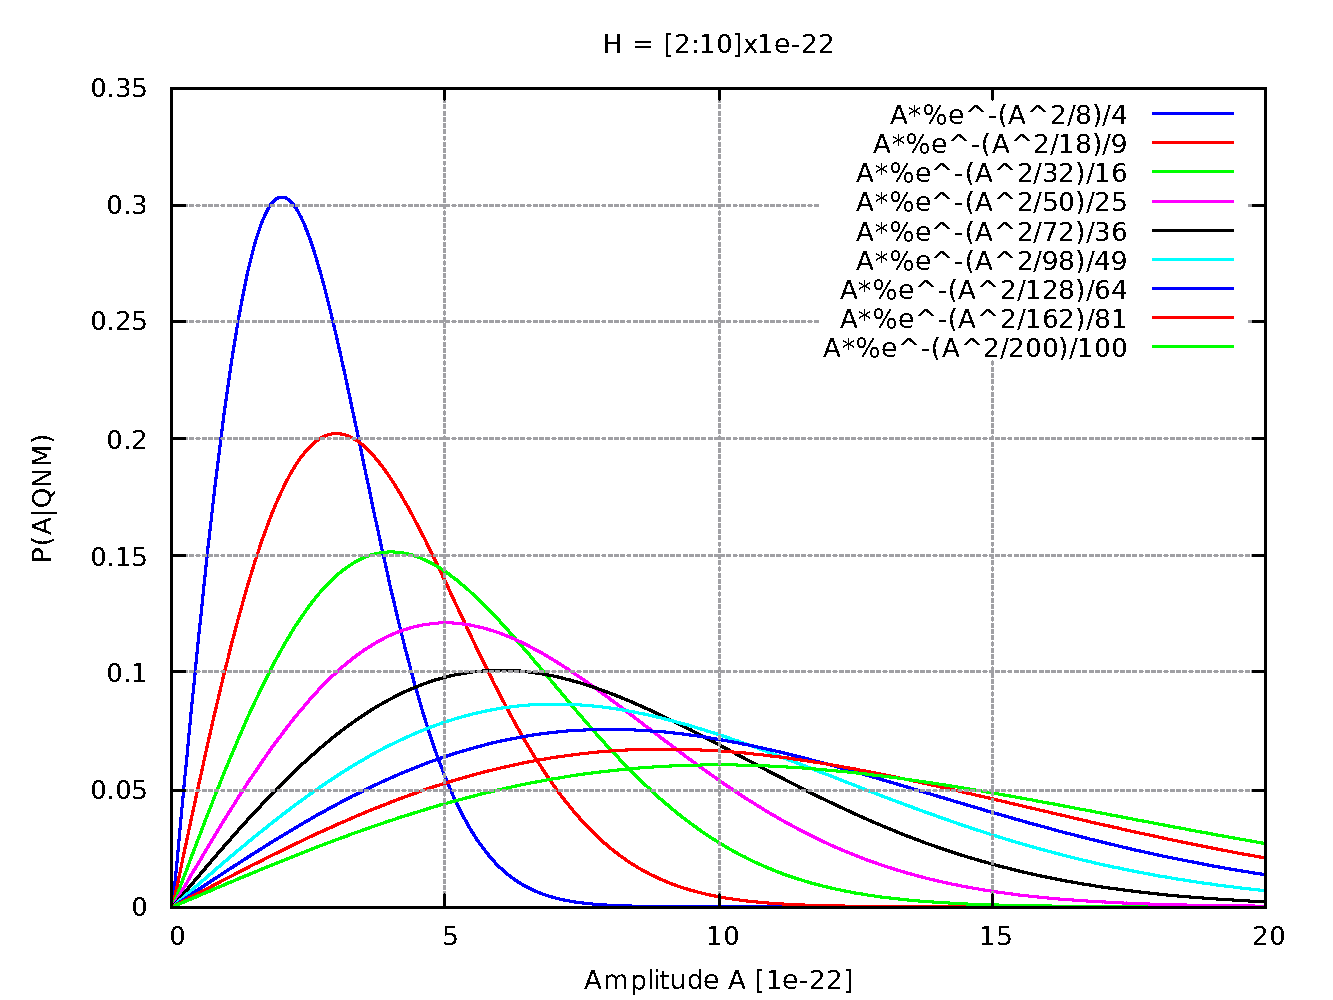
\includegraphics[width=0.5\textwidth]{prior_A.pdf}
  \caption{Amplitude prior (red line) as a hyper-prior (weighted superposition) of several 2D-Gaussian distributions (black lines) with different
    scale parameters $H\in{[2:10]}\times10^{-22}$}
  \label{fig:AmpPrior}
\end{figure}

\subsection{Data preparation}
\label{sec:data-preparation}

Use band-passed 1800s-SFTs (covering GW150914) containing $[10,2000]\,\Hz$ from each detector, band-passed to $[20,1900]\,\Hz$ to avoid boundary
regions where pwelch() PSD estimation trails off.
From this we extracted a $T=8\,$s timeseries $x^X(t)$ centered on the event to analyse.
Time-shifted L1 data by (delaying it by $+7\,\ms$) and multiplied it by $(-1)$ to account for the inverse detector response.
We estimate the (single-sided) PSD $S_X$ by a standard welch method using 8s windows over the 1800s SFT data.

The resulting PSD estimates and data spectra are shown in Fig.~\ref{fig:PSDs}, and the whitened and over-whitened data spectra are shown in
Fig.~\ref{fig:spectra}. Note that the 'data spectra' are only using the data from the $T=8\,$s ``on-source'' window, while the PSD-estimate is done on
the 1800s of original data \emph{excluding} the $T=8\,$s of ``on source'' data.
\begin{figure}[htbp]
  \centering
  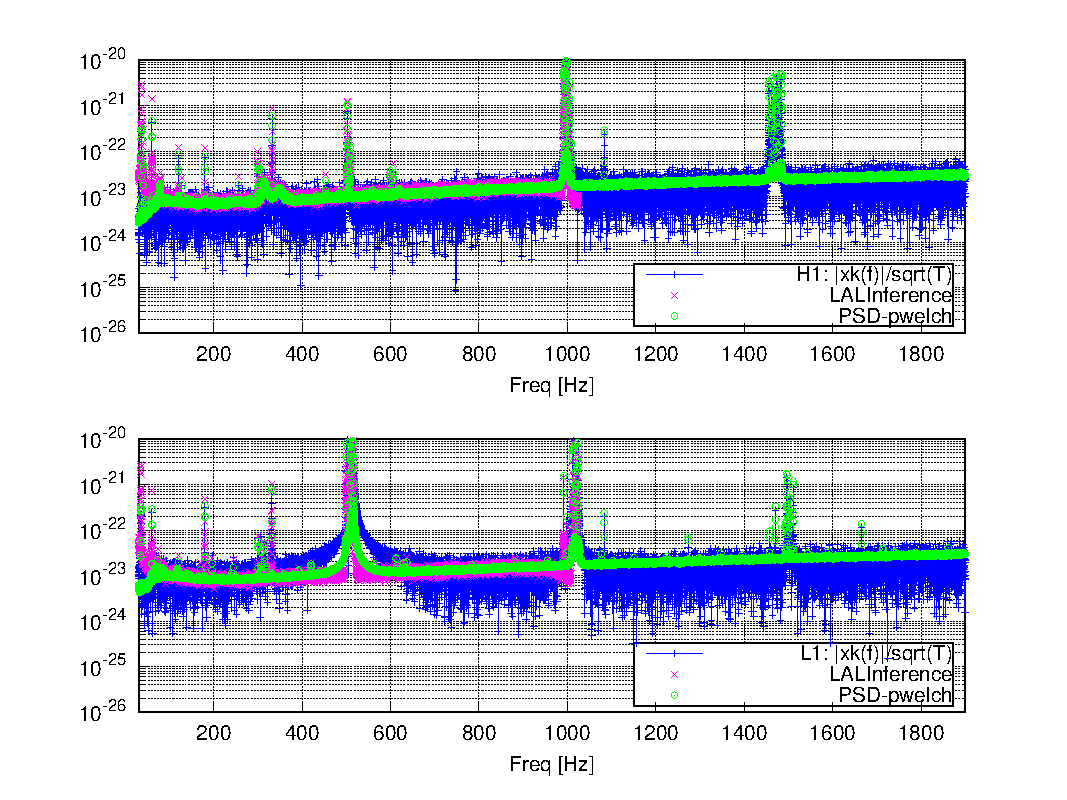
\includegraphics[width=0.75\textwidth,clip]{{\onSourceDir/PSDs}.pdf}
  \caption{Welch PSD estimate of $\sqrt{S_X(f)}$ (green 'o') over $f\in[20,1900]\,\Hz$ on 1800s of data (using an $T=8$s window) for X = H1 (upper plot) and X = L1 (lower plot).
    LALInference PSD-estimate (magenta 'x') and normalized spectrum of $T=8\,$s of data used in the search, i.e. $|\FT{x}^X/\sqrt{T}|$ (blue line and '+').
  }
  \label{fig:PSDs}
\end{figure}
\begin{figure}[htbp]
  \centering
  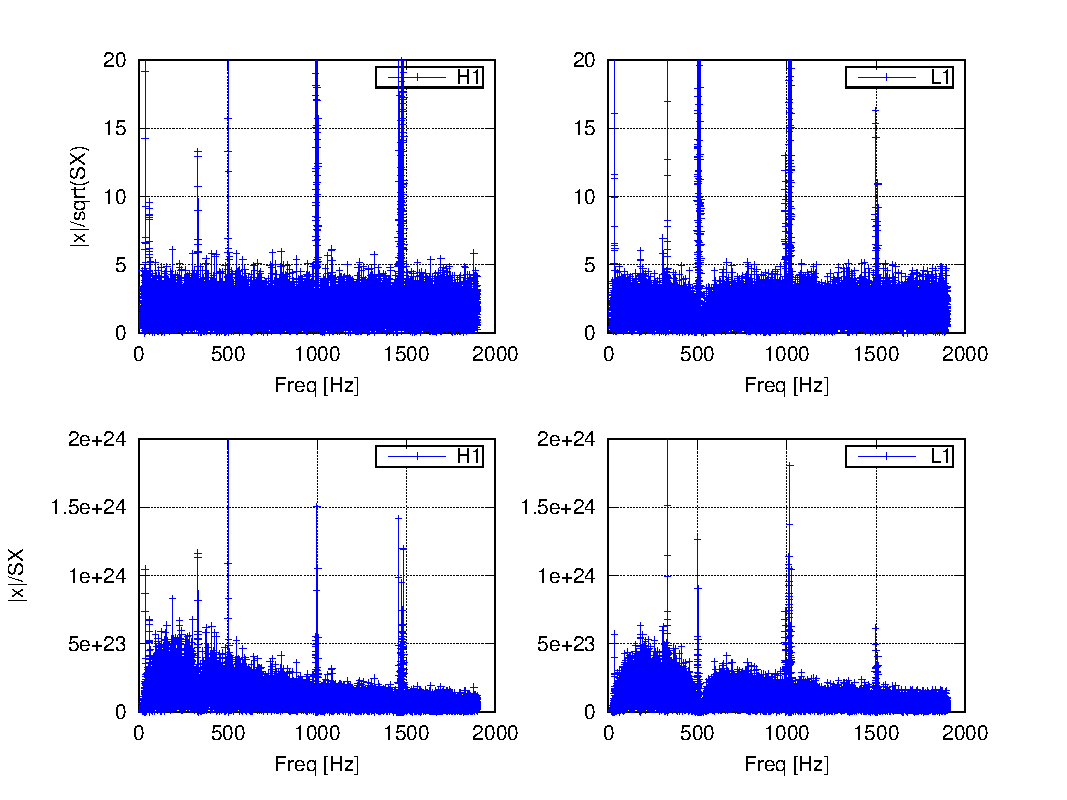
\includegraphics[width=0.75\textwidth,clip]{{\onSourceDir/W-OW-Spectra}.pdf}
  \caption{Whitened $|\FT{x}^X/\sqrt{S_X}|$ (upper row) and over-whitened $|\FT{x}^X/{S_X}|$ (lower row) spectra of $T=8\,$s of data used in the search,
    for X = H1 (left column) and L1 (right column).}
  \label{fig:spectra}
\end{figure}

Although the signal is quite wide-band in frequency domain (see Fig.~\ref{fig:RingdownFT}), in Figs.~\ref{fig:PSDs-zoom} and \ref{fig:spectra-zoom} we
also show a zoom on the most relevant frequency range of ${[200,300]}\,\Hz$.
\begin{figure}[htbp]
  \centering
  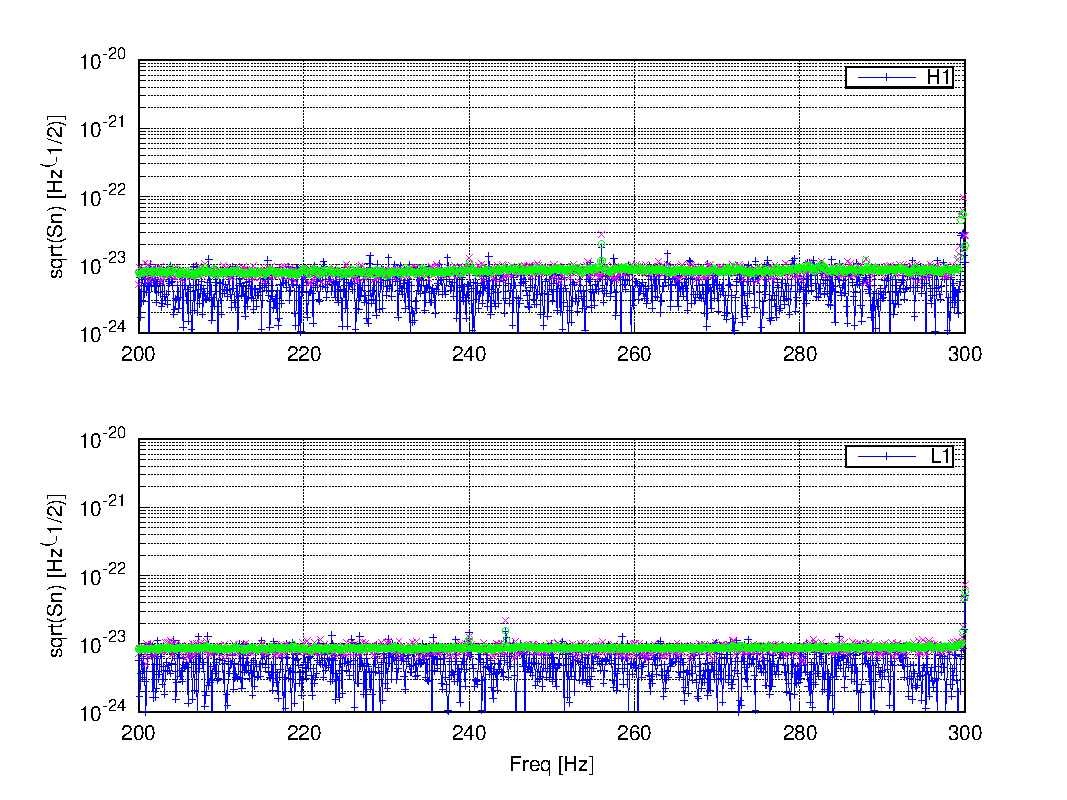
\includegraphics[width=0.75\textwidth,clip]{{\onSourceDir/PSDs-zoom}.pdf}
  \caption{Same as Fig.~\ref{fig:PSDs} but zoomed on frequency range $f\in{[200,300]}\,\Hz$.}
  \label{fig:PSDs-zoom}
\end{figure}
\begin{figure}[htbp]
  \centering
  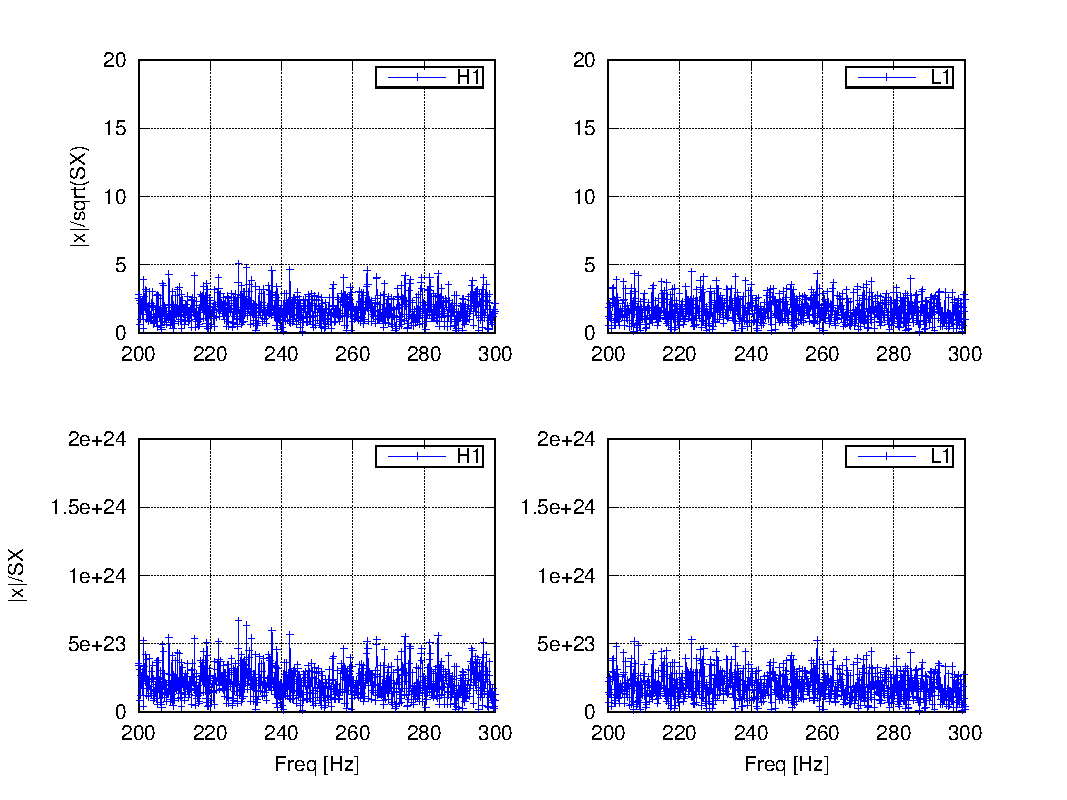
\includegraphics[width=0.75\textwidth,clip]{{\onSourceDir/W-OW-Spectra-zoom}.pdf}
  \caption{Same as Fig.~\ref{fig:spectra} but zoomed on frequency range $f\in{[200,300]}\,\Hz$.}
  \label{fig:spectra-zoom}
\end{figure}


\subsection{Search results on GW150914}
\label{sec:numerical-results}

We search the $\{\freq,\tau\}$ range with uniform priors in $\freq\in{[200,300]}\,\Hz$ and $\tau\in{[0.5,20]}\,\ms$, in steps of $d\freq=0.5\,\Hz$ and
$d\tau=0.5\,\ms$, respectively.
The following plots show snapshots of the posterior at different fixed start-times $\tStart$.
The offset from merger assumes a merger time $\tMerger = 1126259462.423$ (in H1 arrival time), as taken from
\href{https://www.lsc-group.phys.uwm.edu/ligovirgo/cbcnote/TestingGR/O1/G184098/ringdown_presence}{Ian's wiki} and rounded to ms accuracy.
We compute snapshots for different QNM start-times $\tStart - \tMerger$ (referring to H1 arrival times).

\newpage
\parbox{\textwidth}{
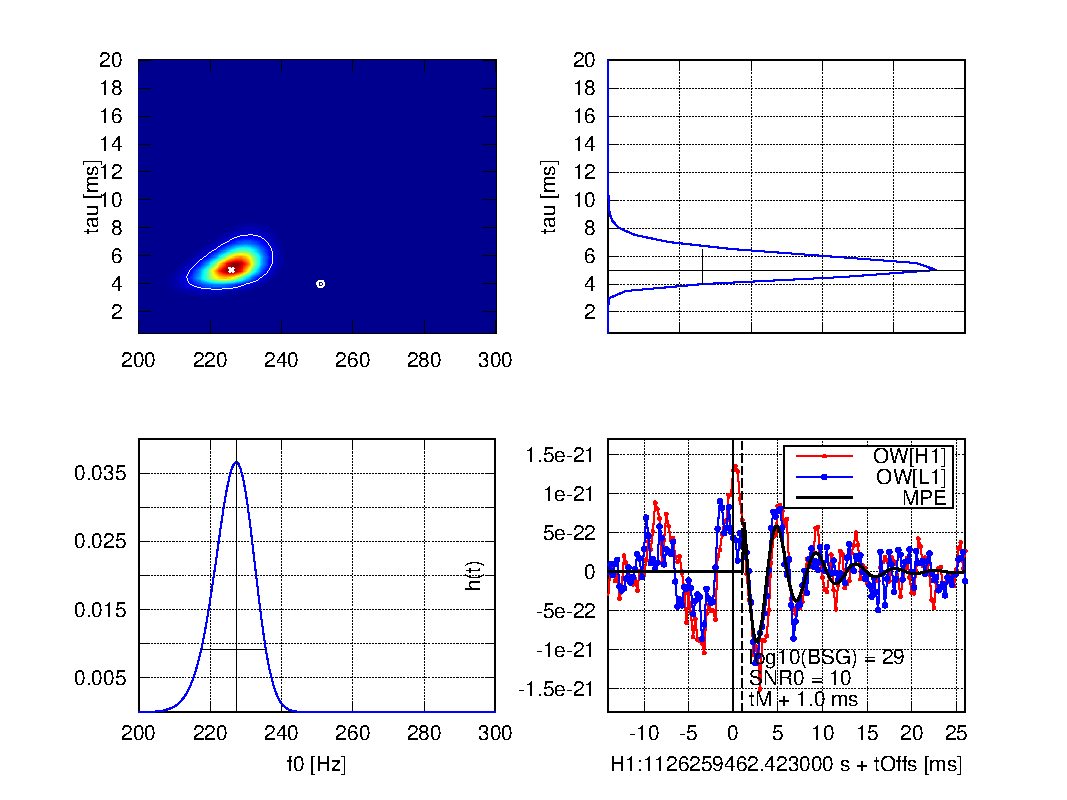
\includegraphics[width=0.9\textwidth]{{\onSourceDir/Search0001-GPS1126259462.424000s-snapshot}.pdf}\\
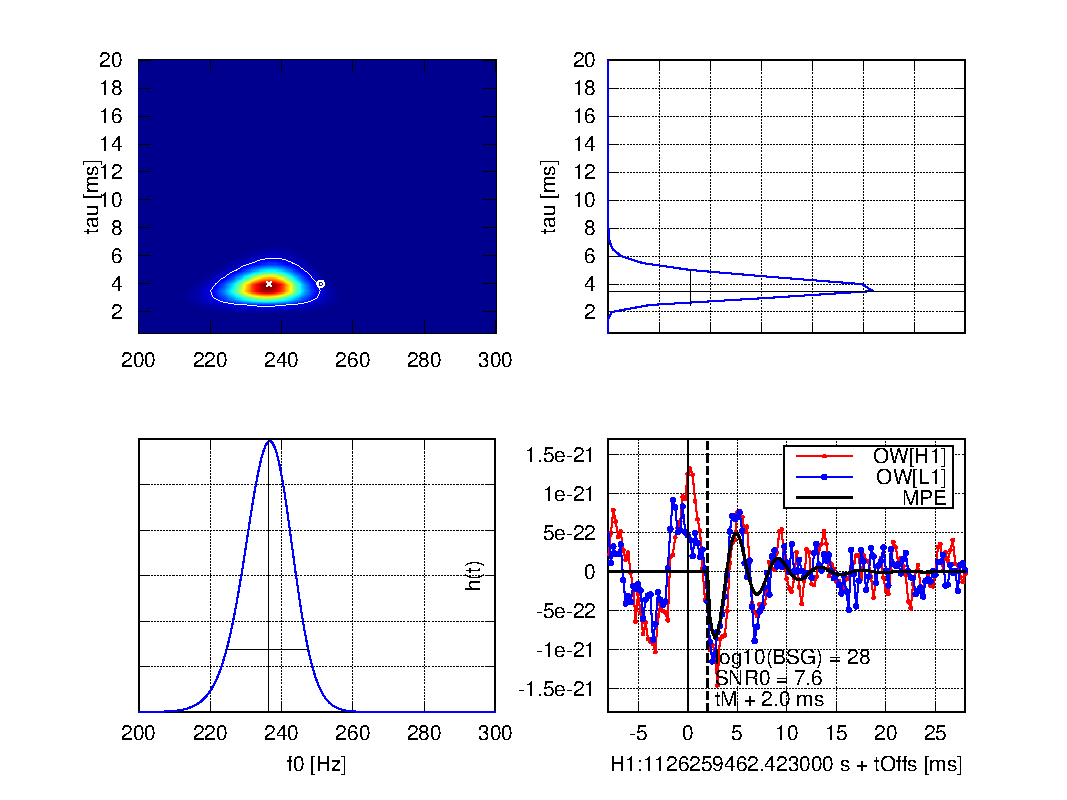
\includegraphics[width=0.9\textwidth]{{\onSourceDir/Search0002-GPS1126259462.425000s-snapshot}.pdf}
}

\newpage
\parbox{\textwidth}{
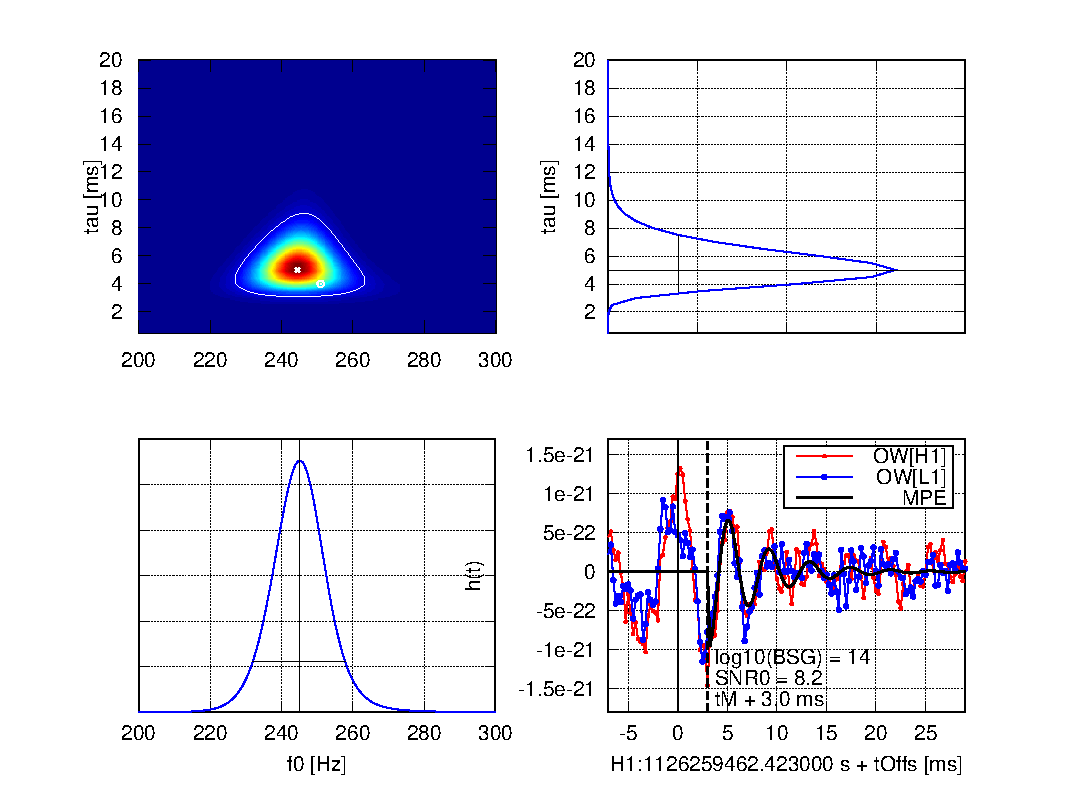
\includegraphics[width=0.9\textwidth]{{\onSourceDir/Search0003-GPS1126259462.426000s-snapshot}.pdf}\\
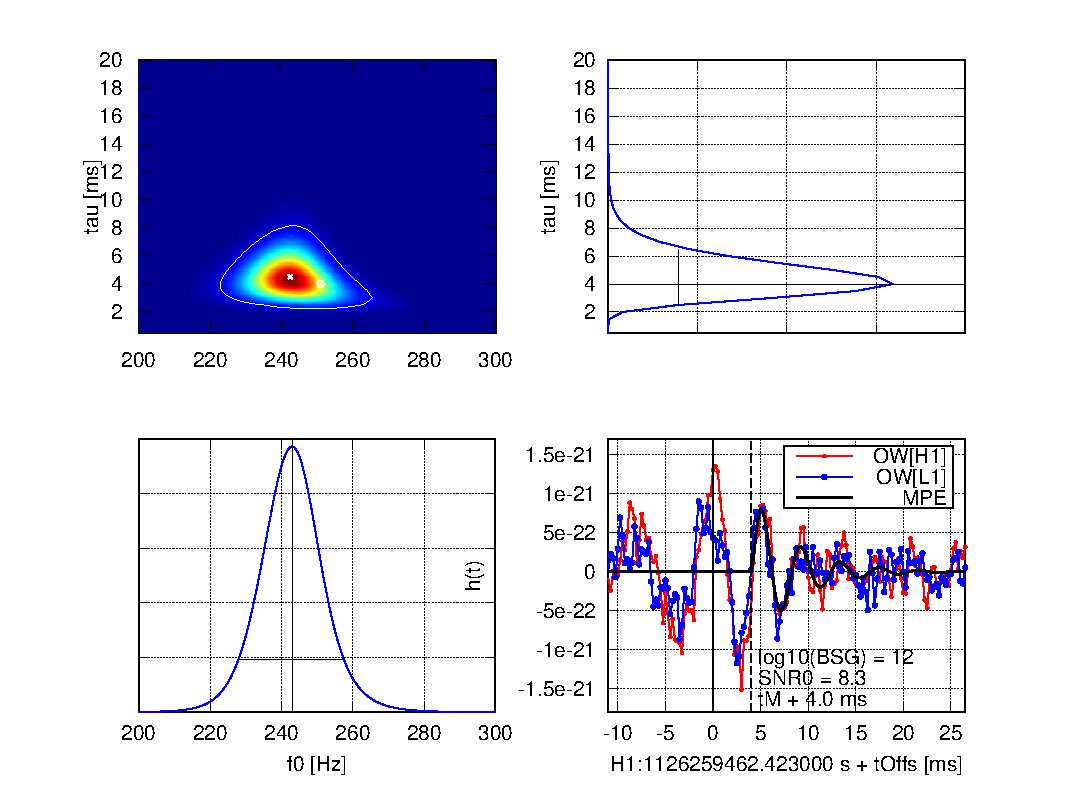
\includegraphics[width=0.9\textwidth]{{\onSourceDir/Search0004-GPS1126259462.427000s-snapshot}.pdf}
}

\newpage
\parbox{\textwidth}{
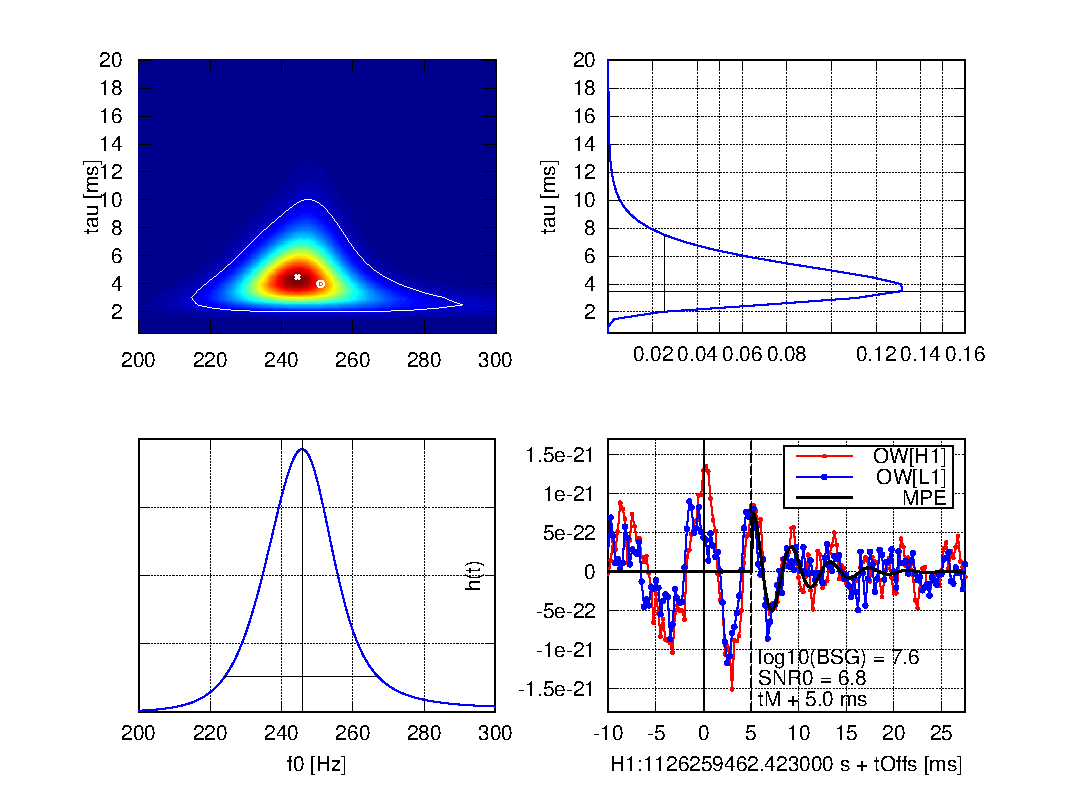
\includegraphics[width=0.9\textwidth]{{\onSourceDir/Search0005-GPS1126259462.428000s-snapshot}.pdf}\\
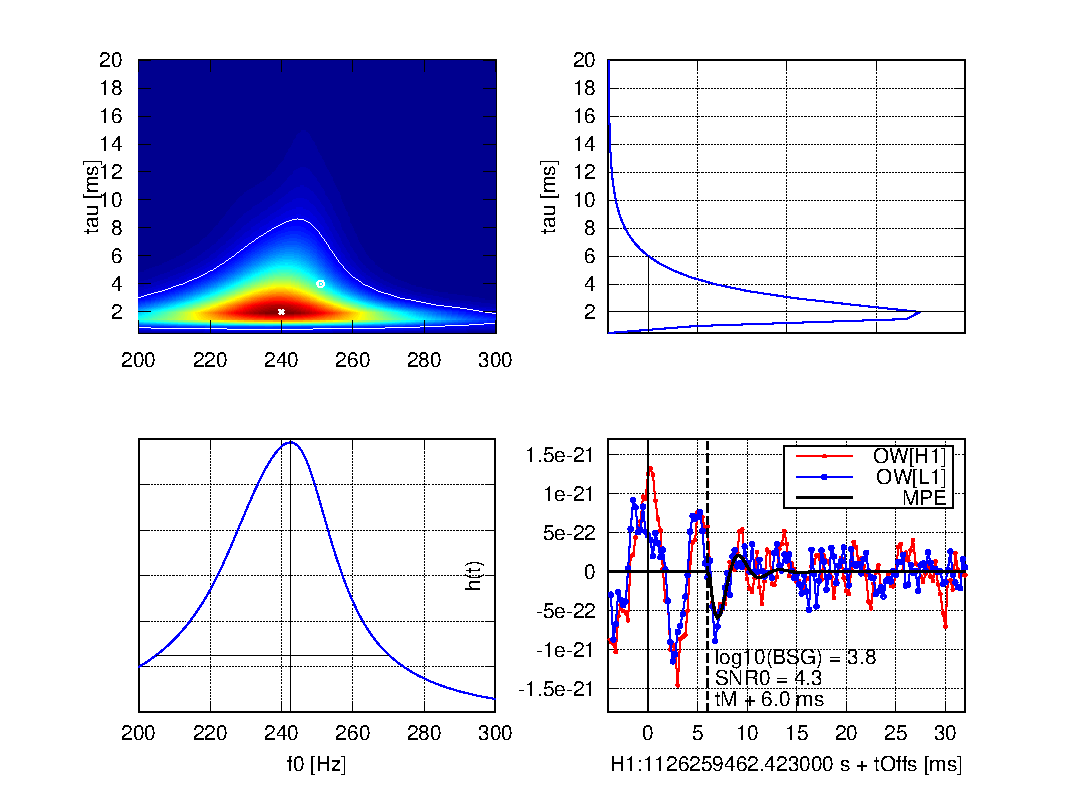
\includegraphics[width=0.9\textwidth]{{\onSourceDir/Search0006-GPS1126259462.429000s-snapshot}.pdf}
}

\newpage
\parbox{\textwidth}{
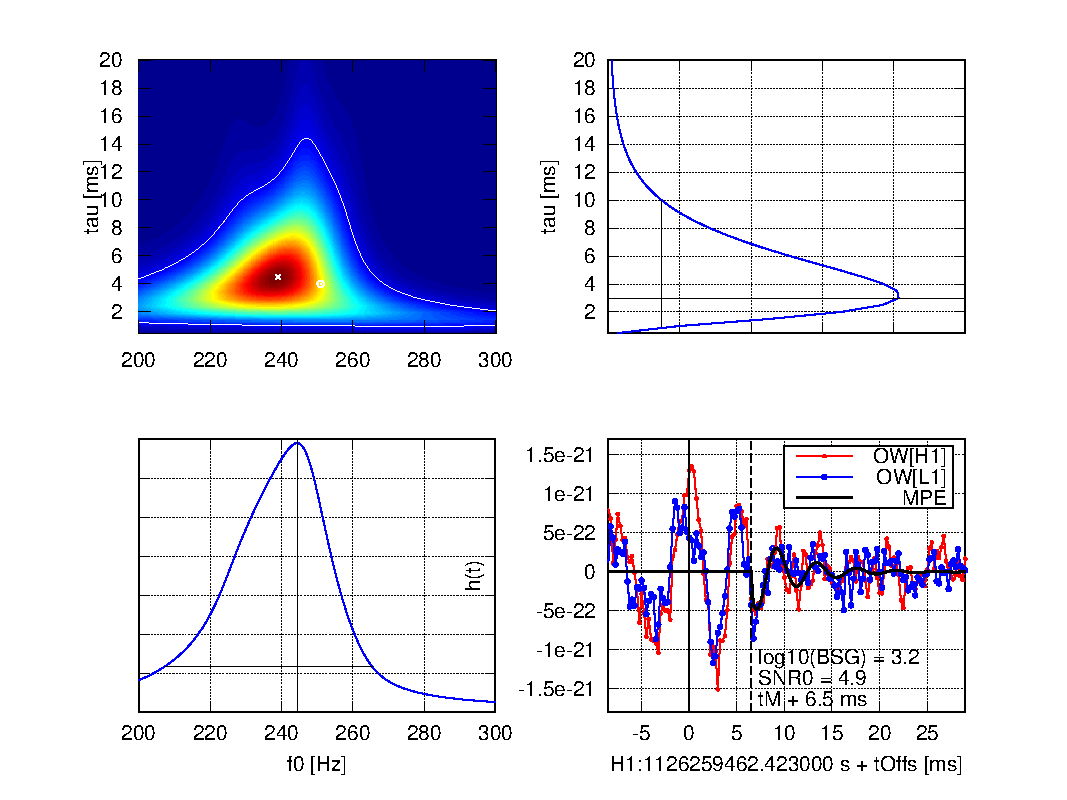
\includegraphics[width=0.9\textwidth]{{\onSourceDir/Search0007-GPS1126259462.429500s-snapshot}.pdf}\\
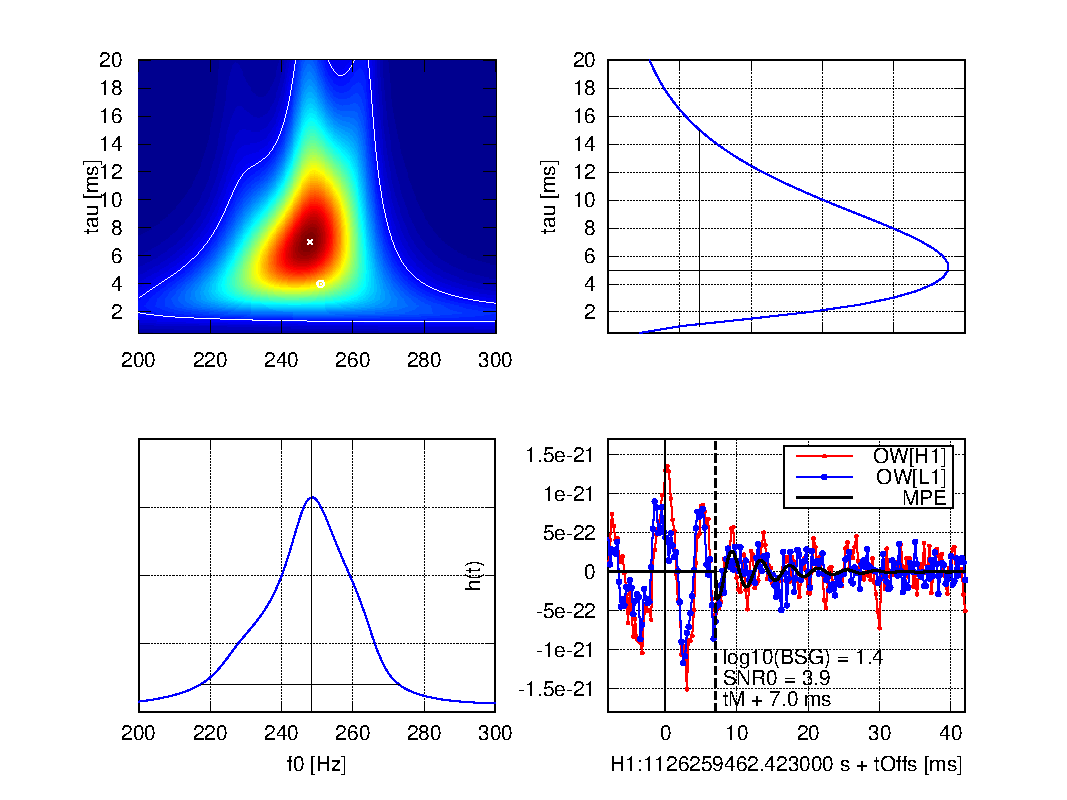
\includegraphics[width=0.9\textwidth]{{\onSourceDir/Search0008-GPS1126259462.430000s-snapshot}.pdf}
}


\newpage
\subsection{Dependence on $\tStart - \tMerger$}
\parbox{\textwidth}{
  \centering
  \includegraphics[width=0.9\textwidth]{{\onSourceDir/t0Evolution}.pdf}
  \includegraphics[width=0.8\textwidth]{{\onSourceDir/Posterior-Contours}.pdf}
}

\section{Testing and characterizing pipeline performance}

\newcommand{\offSourceGaussDir}{./Results/Results-160410-08h29-offSource10000-data20Hz-1900Hz-Prior-f200Hz-300Hz-df0.5Hz-tau0.5ms-20.0ms-dtau0.5ms-H2.0-10.0-dH1.0-injectSqrtSX_8e-24_8e-24}
\newcommand{\offSourceDir}{./Results/Results-160410-10h52-offSource10000-data20Hz-1900Hz-Prior-f200Hz-300Hz-df0.5Hz-tau0.5ms-20.0ms-dtau0.5ms-H2.0-10.0-dH1.0}

\subsection{Off-source searches}
\label{sec:source-searches}
\parbox{\textwidth}{
  We test off-source search performance on Gaussian white noise, as well as on real detector data around GW150914, using
  $10,000$ random start times $\tStart \in \left( {[-3,-0.5]}\,\sec \cup {[0.5,3]}\,\sec\right) + \tMerger$.\\[0.5cm]
  \textbf{Searches in Gaussian noise:}\\[-0.5cm]
  \includegraphics[width=0.8\textwidth]{{\offSourceGaussDir/BSG-hists}.pdf}\\[0.5cm]
  \textbf{Searches in real (off-source) data:}\\[-0.5cm]
  \includegraphics[width=0.8\textwidth]{{\offSourceDir/BSG-hists}.pdf}
}


\newpage
\subsection{Testing parameter-estimation accuracy on injections}
\label{sec:test-param-estim}

We test PE performance on injected QNM signals with perfectly-matched start-time $\tStart$, using $10,000$ random start times
$\tStart \in \left( {[-3,-0.5]}\,\sec \cup {[0.5,3]}\,\sec\right) + \tMerger$.

We consider two cases: (i) QNM parameters drawn from the uniform distributions
$A \in {[3,8]}\times10^{-22}$, $\phi_0 \in {[0,2\pi]}$, $\freq  \in {[200,300]}\,\Hz$, and $\tau \in {[0.5,20]}\,\ms$,
which correspond to the assumed prior distributions for these parameters, except for the amplitude $A$, which has a more complicated (non-flat) prior,
as shown in Fig.~\ref{fig:AmpPrior}.
(ii) QNM parameters with fixed ``GR values'' $\freq =  251\,\Hz,\;\tau = 4\,\ms$, with $A,\phi_0$ drawn randomly as in (i).

In order to avoid injecting a discontinuity at $\tStart$ (which would create problems when band-passing and FFTing the data), we preface the ringdown
with a short ``ringup'' with characteristic timescale $\tau/10$ in the injections, i.e.\
$s(t<\tStart) = A\,e^{10\frac{t-\tStart}{\tau}}\cos\left(2\pi \freq (t-\tStart) + \phi_0\right)$ instead of $s(t<\tStart)=0$ as for the template, as
shown in Fig.~\ref{fig:QNMtemplate}.
\begin{figure}[htbp]
  \centering
  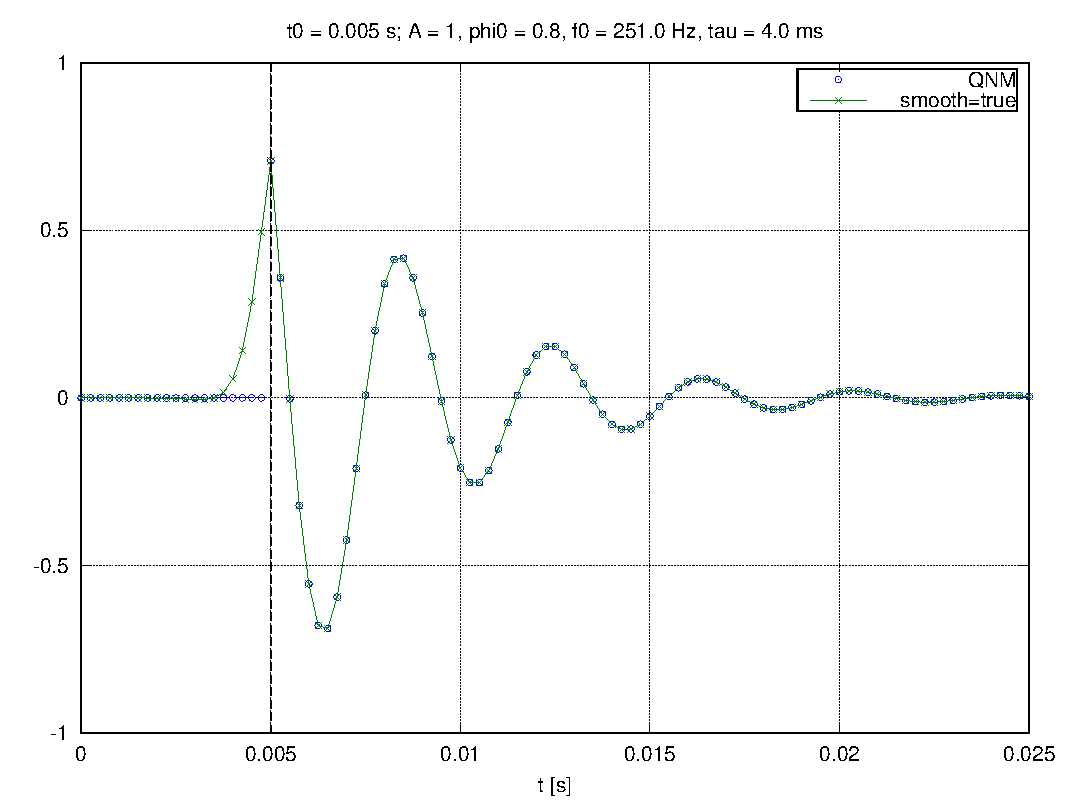
\includegraphics[width=0.5\textwidth]{QNMtemplate.pdf}
  \caption{Example QNM template (labelled 'QNM') used for matching, and ringup+QNM used for injections}
  \label{fig:QNMtemplate}
\end{figure}
We consider 4 injection scenarios:
\begin{enumerate}

\item Pure signals without noise, assuming a white noise-floor of $\sqrt{S_X} = 8\times10^{-24}/\sqrt{\Hz}$.\\[0.2cm]
  These ``signal-only'' injections focus on the accuracy of the MPE estimate versus the true injected parameters, which should essentially be
  perfect at sufficiently large SNR (wrt the assumed noise-floor). For ``lower SNR'' signals, the amplitude prior starts to affect parameter estimation
  and leads to deviations from the injected signal parameters, which is perfectly normal and expected.

\item Signals injected in Gaussian white noise of $\sqrt{S_X} = 8\times10^{-24}/\sqrt{\Hz}$, assuming this exact noise PSD.\\[0.2cm]
  The injections into \emph{known} Gaussian noise exactly realize all of the assumptions, and as we're drawing signals essentially from the
  priors, we expect the parameter posteriors to accurately predict their frequency of coverage \citep[e.g.\ see][]{2008arXiv0804.1161S}.

\item Signals injected in Gaussian white noise of $\sqrt{S_X} = 8\times10^{-24}/\sqrt{\Hz}$, estimating PSD from the data.\\[0.2cm]
  Compared to the previous case this basically just tests the reliability of noise-estimation, and we're still expecting posteriors to predict their
  coverage.

\item Signals injected into real off-source detector data.\\[0.2cm]
  Here we can quantify how much of an effect ``real noise'' instead of Gaussian noise has on the coverage of the posteriors, which can lead to over-
  or under-coverage.

\end{enumerate}

Cases 1-3 essentially serve to test self-consistency of the method and implementation, given that we know exactly what to expect, i.e.\ in order to
catch mistakes or bugs. Case 4 serves to test the validity of our assumptions (mostly about the noise) in real detector data.

\newcommand{\InjSignalOnlyPriorRangesDir}{./Results/Results-160408-19h21-injections10000-data20Hz-1900Hz-Prior-f200Hz-300Hz-df0.5Hz-tau0.5ms-20.0ms-dtau0.5ms-H2.0-10.0-dH1.0-injectPriorRanges-injectSqrtSX_0_0-assumeSqrtSX_8e-24_8e-24}
\newcommand{\InjKnownGaussPriorRangesDir}{./Results/Results-160408-21h14-injections10000-data20Hz-1900Hz-Prior-f200Hz-300Hz-df0.5Hz-tau0.5ms-20.0ms-dtau0.5ms-H2.0-10.0-dH1.0-injectPriorRanges-injectSqrtSX_8e-24_8e-24-assumeSqrtSX_8e-24_8e-24}
\newcommand{\InjUnknownGaussPriorRangesDir}{./Results/Results-160408-23h07-injections10000-data20Hz-1900Hz-Prior-f200Hz-300Hz-df0.5Hz-tau0.5ms-20.0ms-dtau0.5ms-H2.0-10.0-dH1.0-injectPriorRanges-injectSqrtSX_8e-24_8e-24}
\newcommand{\InjOffSourcePriorRangesDir}{./Results/Results-160409-01h00-injections10000-data20Hz-1900Hz-Prior-f200Hz-300Hz-df0.5Hz-tau0.5ms-20.0ms-dtau0.5ms-H2.0-10.0-dH1.0-injectPriorRanges}

\newpage
\subsubsection{Case 1(i): Prior-range $\{\freq,\tau\}$ injections, signal-only with assumed white noise}
\label{sec:case-1:injections-signal-only}

  \begin{figure}[htbp]
    \centering
    \includegraphics[width=0.75\textwidth]{{\InjSignalOnlyPriorRangesDir/Injections-PE-errors}.pdf}
    \caption{MP estimation errors (top 2 rows), recovered SNR (bottom left) and Bayes-factor (bottom right) as functions of injected SNR. Solid line denotes the median, error-bars denote $\pm25\%$-ile and dashed lines are $2.5\%$- and $97.5\%$-iles, respectively.}
    \label{fig:PEerrors-1i}
  \end{figure}

  \begin{figure}[htbp]
    \centering
    \includegraphics[width=0.55\textwidth]{{\InjSignalOnlyPriorRangesDir/Injections-PE-coverage}.pdf}
    \caption{Posterior coverage versus percentile ("pp-plot"), showing mean (solid line) and $90\%$-credible interval (green).}
    \label{fig:pp-case-1i}
  \end{figure}


\newpage
\subsubsection{Case 2(i): Prior-range $\{\freq,\tau\}$ injections, \textbf{known} Gaussian white noise}
\label{sec:case-2:injections-known-Gauss}

\parbox{\textwidth}{
  \includegraphics[width=0.9\textwidth]{{\InjKnownGaussPriorRangesDir/Injections-PE-errors}.pdf}\\
  \includegraphics[width=0.9\textwidth]{{\InjKnownGaussPriorRangesDir/Injections-PE-coverage}.pdf}
}

\newpage
\subsubsection{Case 3(i): Prior-range $\{\freq,\tau\}$ injections, \textbf{unknown} Gaussian white noise}
\label{sec:case-3:injections-unknown-Gauss}

\parbox{\textwidth}{
  \includegraphics[width=0.9\textwidth]{{\InjUnknownGaussPriorRangesDir/Injections-PE-errors}.pdf}\\
  \includegraphics[width=0.9\textwidth]{{\InjUnknownGaussPriorRangesDir/Injections-PE-coverage}.pdf}
}

\newpage
\subsubsection{Case 4(i): Prior-range $\{\freq,\tau\}$ injections, off-source detector data}
\label{sec:case-4:injections-real-noise}

\parbox{\textwidth}{
  \includegraphics[width=0.9\textwidth]{{\InjOffSourcePriorRangesDir/Injections-PE-errors}.pdf}\\
  \includegraphics[width=0.9\textwidth]{{\InjOffSourcePriorRangesDir/Injections-PE-coverage}.pdf}
}

\newpage
\subsubsection{Case 1(ii): fixed-$\{\freq=251\Hz,\tau=4\ms\}$ injections, signal-only with assumed white noise}
\label{sec:case-1:injections-signal-only}

\newcommand{\InjSignalOnlyIMRDir}{./Results/Results-160409-02h53-injections10000-data20Hz-1900Hz-Prior-f200Hz-300Hz-df0.5Hz-tau0.5ms-20.0ms-dtau0.5ms-H2.0-10.0-dH1.0-injectIMR-injectSqrtSX_0_0-assumeSqrtSX_8e-24_8e-24}
\newcommand{\InjKnownGaussIMRDir}{./Results/Results-160409-04h46-injections10000-data20Hz-1900Hz-Prior-f200Hz-300Hz-df0.5Hz-tau0.5ms-20.0ms-dtau0.5ms-H2.0-10.0-dH1.0-injectIMR-injectSqrtSX_8e-24_8e-24-assumeSqrtSX_8e-24_8e-24}
\newcommand{\InjUnknownGaussIMRDir}{./Results/Results-160409-06h39-injections10000-data20Hz-1900Hz-Prior-f200Hz-300Hz-df0.5Hz-tau0.5ms-20.0ms-dtau0.5ms-H2.0-10.0-dH1.0-injectIMR-injectSqrtSX_8e-24_8e-24}
\newcommand{\InjOffSourceIMRDir}{./Results/Results-160409-08h32-injections10000-data20Hz-1900Hz-Prior-f200Hz-300Hz-df0.5Hz-tau0.5ms-20.0ms-dtau0.5ms-H2.0-10.0-dH1.0-injectIMR}

\parbox{\textwidth}{
  \includegraphics[width=0.9\textwidth]{{\InjSignalOnlyIMRDir/Injections-PE-errors}.pdf}\\
  \includegraphics[width=0.9\textwidth]{{\InjSignalOnlyIMRDir/Injections-PE-coverage}.pdf}
}

\newpage
\subsubsection{Case 2(ii): fixed-$\{\freq=251\Hz,\tau=4\ms\}$ injections, \textbf{known} Gaussian white noise}
\label{sec:case-2:injections-known-Gauss}

\parbox{\textwidth}{
  \includegraphics[width=0.9\textwidth]{{\InjKnownGaussIMRDir/Injections-PE-errors}.pdf}\\
  \includegraphics[width=0.9\textwidth]{{\InjKnownGaussIMRDir/Injections-PE-coverage}.pdf}
}

\newpage
\subsubsection{Case 3(ii): fixed-$\{\freq=251\Hz,\tau=4\ms\}$ injections, \textbf{unknown} Gaussian white noise}
\label{sec:case-3:injections-unknown-Gauss}

\parbox{\textwidth}{
  \includegraphics[width=0.9\textwidth]{{\InjUnknownGaussIMRDir/Injections-PE-errors}.pdf}\\
  \includegraphics[width=0.9\textwidth]{{\InjUnknownGaussIMRDir/Injections-PE-coverage}.pdf}
}

\newpage
\subsubsection{Case 4(ii): fixed-$\{\freq=251\Hz,\tau=4\ms\}$ injections, off-source detector data}
\label{sec:case-4:injections-real-noise}

\parbox{\textwidth}{
  \includegraphics[width=0.9\textwidth]{{\InjOffSourceIMRDir/Injections-PE-errors}.pdf}\\
  \includegraphics[width=0.9\textwidth]{{\InjOffSourceIMRDir/Injections-PE-coverage}.pdf}
}


\newpage

\subsection{Varying noise-realization at fixed-$\{\freq=251\Hz,\tau=4\ms, A = 2.5\times10^{21}, \phi_0 = 0\}$ injection}
\label{sec:varying-tstart-at}

\newcommand{\onInjectionDir}{./Results/Results-160410-11h03-onInjection11-data20Hz-1900Hz-Prior-f200Hz-300Hz-df0.5Hz-tau0.5ms-20.0ms-dtau0.5ms-H2.0-10.0-dH1.0-injectSqrtSX_8e-24_8e-24}
\begin{figure}[htbp]
  \vspace*{-1cm}
  \includegraphics[width=0.8\textwidth]{{\onInjectionDir/t0Evolution}.pdf}\\[-0.7cm]
  \includegraphics[width=0.8\textwidth]{{\onInjectionDir/Posterior-Contours}.pdf}
  \caption{Example 1 in Gaussian noise}
\end{figure}

\renewcommand{\onInjectionDir}{./Results/Results-160410-11h04-onInjection11-data20Hz-1900Hz-Prior-f200Hz-300Hz-df0.5Hz-tau0.5ms-20.0ms-dtau0.5ms-H2.0-10.0-dH1.0-injectSqrtSX_8e-24_8e-24}
\begin{figure}[htbp]
  \includegraphics[width=0.9\textwidth]{{\onInjectionDir/t0Evolution}.pdf}
  \includegraphics[width=0.8\textwidth]{{\onInjectionDir/Posterior-Contours}.pdf}
  \caption{Example 2 in Gaussian noise}
\end{figure}

\renewcommand{\onInjectionDir}{./Results/Results-160410-11h06-onInjection11-data20Hz-1900Hz-Prior-f200Hz-300Hz-df0.5Hz-tau0.5ms-20.0ms-dtau0.5ms-H2.0-10.0-dH1.0-injectSqrtSX_8e-24_8e-24}
\begin{figure}[htbp]
  \includegraphics[width=0.9\textwidth]{{\onInjectionDir/t0Evolution}.pdf}
  \includegraphics[width=0.8\textwidth]{{\onInjectionDir/Posterior-Contours}.pdf}
  \caption{Example 3 in Gaussian noise}
\end{figure}


\renewcommand{\onInjectionDir}{./Results/Results-160410-11h23-onInjection11-data20Hz-1900Hz-Prior-f200Hz-300Hz-df0.5Hz-tau0.5ms-20.0ms-dtau0.5ms-H2.0-10.0-dH1.0}
\begin{figure}[htbp]
  \includegraphics[width=0.9\textwidth]{{\onInjectionDir/t0Evolution}.pdf}
  \includegraphics[width=0.8\textwidth]{{\onInjectionDir/Posterior-Contours}.pdf}
  \caption{Example 1 in real off-source data}
\end{figure}

\renewcommand{\onInjectionDir}{./Results/Results-160410-11h24-onInjection11-data20Hz-1900Hz-Prior-f200Hz-300Hz-df0.5Hz-tau0.5ms-20.0ms-dtau0.5ms-H2.0-10.0-dH1.0}
\begin{figure}[htbp]
  \includegraphics[width=0.9\textwidth]{{\onInjectionDir/t0Evolution}.pdf}
  \includegraphics[width=0.8\textwidth]{{\onInjectionDir/Posterior-Contours}.pdf}
  \caption{Example 2 in real off-source data}
\end{figure}


\renewcommand{\onInjectionDir}{./Results/Results-160410-11h26-onInjection11-data20Hz-1900Hz-Prior-f200Hz-300Hz-df0.5Hz-tau0.5ms-20.0ms-dtau0.5ms-H2.0-10.0-dH1.0}
\begin{figure}[htbp]
  \includegraphics[width=0.9\textwidth]{{\onInjectionDir/t0Evolution}.pdf}
  \includegraphics[width=0.8\textwidth]{{\onInjectionDir/Posterior-Contours}.pdf}
  \caption{Example 3 in real off-source data}
\end{figure}


\newpage
\appendix

\section{Deprecated old way to compute $\scalar{s}{s}$: const noise floor + time-domain integration}
\label{sec:depr-first-way}

Given that aLIGO noise-curve is relatively ``white'' over a broad-band in the ``bucket'', and the signal $s(t)$ of Eq.~\eqref{eq:1} can still be
considered relatively ``narrow band'' ($\sim \pm 100\Hz$) with respect to this noise curve, we can approximate the signal-normalization integral as
\begin{align}
  \label{eq:17}
  \scalar{s}{s} &= \sum_X 2 \int_{-\infty}^{\infty} \frac{\FT{s}^X(f)\,\FT{s}^{*X}(f)}{S_X(f)}\,d f\\
  &\sim \sum_X \frac{2}{S_X(f')} \, \int_{0}^{\infty} s^2(t;\parA,\parE)\,dt\\
  & = \frac{2\,\Ndet}{\Sn(f')} \,\int \left( \As^2\,\hs^2(t) + 2\As\Ac\,\hs\hc + \Ac^2\,\hc^2\right)\,d t\\
  & = \parA \cdot \M \,\cdot\parA\,,
\end{align}
with
\begin{equation}
  \label{eq:23}
  \M \equiv
  2\Ndet \begin{pmatrix}
    \Is  & \Isc \\
    \Isc  & \Ic\\
  \end{pmatrix}
\end{equation}
with
\begin{align}
  \label{eq:43}
  \Is  &\equiv \frac{1}{\Sn(f')}\int_0^\infty e^{-\frac{2t}{\tau}}\,\sin^2(2\pi f t)\,dt = \frac{1}{2\pi f}\int e^{-\frac{\varphi}{Q}} \sin^2\!\varphi\,d\varphi\\
  \Ic  &\equiv \int_0^\infty e^{-\frac{2t}{\tau}}\,\cos^2(2\pi f t)\,dt = \frac{1}{2\pi f}\int e^{-\frac{\varphi}{Q}} \cos^2\!\varphi\,d\varphi\\
  \Isc &\equiv \int_0^\infty e^{-\frac{2t}{\tau}}\,\sin(2\pi f t)\cos(2\pi f t)\,dt = \frac{1}{4\pi f}\int e^{-\frac{\varphi}{Q}} \sin2\varphi\,d\varphi\,,
\end{align}
where $f'$ is some (unknown) frequency within the effective frequency band around the central signal frequency $f$ (using mean-value theorem), and we
have used the assumption of identical signal model in both detectors (after time-shifting the data and correcting for antenna-pattern differences).

The respective integrals to compute are
\begin{align}
  \label{eq:18}
\end{align}
using the definitions
\begin{align}
  \label{eq:3}
  \varphi &\equiv 2\pi f \Dt\,,\\
  Q       &\equiv \pi f \tau\,.
\end{align}
Assuming only non-critically damped signals, i.e. $Q\gtrsim \Ord{\pi}$, these integrals can be approximated computed analytically as
\begin{align}
  \label{eq:19}
  \Is' &= \left. \frac{-1}{2\pi f}\frac{Q^2}{1 + 4Q^2}e^{-\frac{\varphi}{Q}}\left[ \sin2\varphi + 2Q + \frac{\sin^2\varphi}{Q}\right]\right|_0^\infty
  = \frac{2Q}{2\pi f}\,\frac{Q^2}{1+4Q^2}
  = \frac{\tau}{4 + Q^{-2}} \\
  & \stackrel{Q\gg1}{\approx} \frac{\tau}{4}\,,\\
  \Ic' &= \left. \frac{-1}{2\pi f}\frac{Q^2}{1 + 4Q^2}e^{-\frac{\varphi}{Q}}\left[ -\sin2\varphi + 2Q + \frac{\cos^2\varphi}{Q}\right]\right|_0^\infty
  = \frac{2Q + \frac{1}{Q}}{2\pi f}\,\frac{Q^2}{1+4Q^2} = \frac{\tau}{4}\,\left(\frac{2 + Q^{-2}}{2 + Q^{-2}/2}\right) \\
  & \stackrel{Q\gg1}{\approx} \frac{\tau}{4}\,,\\
  \Isc' &= \left. \frac{-1}{2\pi f}\frac{Q^2}{1 + 4Q^2}e^{-\frac{\varphi}{Q}}\left[ 2\cos^2\varphi - 1 + \frac{\sin2\varphi}{2Q}\right]\right|_0^\infty
  = \frac{1}{2\pi f}\,\frac{Q^2}{1+4Q^2} = \frac{\tau}{8Q\,(1 + Q^{-2}/4)}\\
  &\stackrel{Q\gg1}{\approx} \frac{1}{2Q}\,\Is \ll \Is \approx 0\,.
\end{align}
So $\Is \approx \Ic \approx \frac{\Ndet\tau}{2\Sn(f')}$ and $\Isc\approx 0$, and we obtain the approximate $\M$-matrix as
\begin{equation}
  \label{eq:42}
  \M \approx \frac{\Ndet\,\tau}{2\Sn(f')}\,\eye = \begin{pmatrix} I_0 & 0 \\ 0 & I_0 \end{pmatrix}\,.
\end{equation}
Note: in the QNM search we'll approximate $\Sn(f')$ in this expression by the arithmetic mean $\langle\Sn(f)\rangle_{f\pm\Delta f}$ around each
template frequency $f$. This fixed-SN high-Q limit was originally used in the \href{https://dcc.ligo.org/LIGO-G1600153-v1}{v1} of this search and
document, which was originally circulated.

\bibliography{RingdownSearch}

\end{document}

%%% Local Variables:
%%% ispell-local-dictionary: "american"
%%% fill-column: 150
%%% mode: latex
%%% mode: flyspell
%%% TeX-master: t
%%% End:
